\documentclass[a4paper,12pt]{article} 
% 使用ctex包支持中文
\usepackage[UTF8,heading = true]{ctex}
\usepackage[utf8]{inputenc}
\usepackage[T1]{fontenc}
\usepackage{graphicx}
\usepackage{float}
\usepackage{amsmath}
\usepackage{amsfonts}
\usepackage{amssymb}
\usepackage{booktabs}
\usepackage{multirow}
\usepackage{subcaption}
\usepackage{indentfirst}
\usepackage{geometry}
\usepackage{fancyhdr}
\usepackage{ctex}
\usepackage[labelfont=bf]{caption}
\usepackage{listings}
\usepackage{xcolor} % 用于定义自定义颜色和高亮
\usepackage{ragged2e} % 导入ragged2e宏包,用于支持段落两端对齐
\usepackage{cite}

\lstset{
  language=Matlab,              % 设置语言为 MATLAB
  basicstyle=\ttfamily\small,   % 设置基本样式
  keywordstyle=\color{blue},    % 设置关键字样式
  stringstyle=\color{red},      % 设置字符串样式
  commentstyle=\color{green},   % 设置注释样式
  morecomment=[l][\color{magenta}]{\%},   % 对行内注释进行高亮
  morecomment=[s][\color{magenta}]{\%\{}{\%\}},   % 对多行注释进行高亮
  frame=single,                 % 给代码添加框
  rulecolor=\color{black},      % 框的颜色
  numbers=left,                 % 在左侧添加行号
  numberstyle=\tiny\color{gray},% 行号样式
  breaklines=true,              % 自动换行
  postbreak=\mbox{\textcolor{red}{$\hookrightarrow$}\space},
  showstringspaces=false,       % 不特别显示字符串中的空格
  tabsize=2                     % 设置tab为2个空格宽度
}



\geometry{left=3cm,right=3cm,top=3cm,bottom=3cm}

%\ctexset{
    % 修改 section。
    %section={   
        %name={实验,:},
        %number={\chinese{section}},
        %format=\heiti\bfseries\centering\zihao{-2} % 设置 section 标题为黑体、右对齐、小4号字
    %},
    % 修改 subsection。
    %subsection={   
        %name={,、},
        %number={\chinese{subsection}},
        %format=\songti\bfseries\zihao{4} % 设置 subsection 标题为黑体、5号字
    %},
    % 修改 subsection。
    %subsubsection={   
        %name={,、},
        %number={\arabic{subsubsection}},
        %format=\songti\bfseries\zihao{-4} % 设置 subsection 标题为黑体、5号字
    %}
%}
\fancyhead{}


\begin{document}

%制作封面
\begin{titlepage}
    \begin{center}
        \par
            \centerline{
\includegraphics[scale=1.5]{data/media/image1.jpeg} 
\includegraphics[scale=3]{data/media/image2.jpeg}} %插入图片
        \par
		\vskip 5cm
		\lishu \fontsize{50}{20} 实\quad 验\quad 报\quad 告
  
		\vskip 2cm
        \lishu \fontsize{35}{20} 实\quad 验\quad 一
        \vskip 5cm

	\begin{tabular}{l}
		\songti \zihao{-2} \bfseries 课程名称:《数字信号处理实验》
		\quad \\
	    	\songti \zihao{-2} \bfseries 学生姓名:ZYH
	    	\quad \\
		\songti \zihao{-2} \bfseries 学生学号:202264691103
		\quad \\
	    	\songti \zihao{-2} \bfseries 学生专业:人工智能
	    	\quad \\
	     \songti \zihao{-2} \bfseries 开课学期:2023-2024年第二学期
	     \quad \\
           \songti \zihao{-2} \bfseries  提交日期:2024年5月8日
    \end{tabular}
    \end{center}
\end{titlepage}


% 生成目录
\newpage
\pagestyle{empty}
\begin{center}
\tableofcontents
\end{center}

\newpage

\setcounter{page}{1}

\section{验证性实验}
\subsection{实验目的}
\begin{itemize}
    \item 熟悉使用MATLAB 在时域中产生一些基本的离散时间信号
    \item 讨论正弦序列、复指数序列的性质
    \item 学习方波、锯齿波和sinc函数并绘图
    \item 熟悉利用函数$y = filter(p,d,x)$实现差分方程的仿真
    \item 熟悉用函数$y = conv(x,h)$计算卷积
    \item 熟悉用filter函数计算卷积
    \item 使用不同函数求解系统冲激与阶跃响应
    \cite{ning2012}
\end{itemize}



\subsection{实验原理}

\subsubsection{MATLAB基本的离散时间信号}
\begin{itemize}
    \item 单位抽样序列

    单位抽样序列是一种在离散时间点上取值为1,在其他时间点上取值为0的序列。其原理是在离散时间轴上,只在原点处存在一个取值为1的样本,其他位置均为0。单位抽样序列在离散时间系统中常用于表示瞬时事件或者作为信号的激励。
    
    \item 单位阶跃序列

    单位阶跃序列是一种在离散时间点上取值为1,在之前的所有时间点上取值为1的序列。其原理是在离散时间轴上,从原点开始,一直取值为1,表示系统在原点之前一直处于稳态,然后在原点处发生突变。单位阶跃序列在离散时间系统中常用于表示系统的初始条件或者作为信号的激励。

    \item 正弦序列
    
    正弦序列是一种以离散时间为自变量的正弦函数。其原理是根据离散时间的取值,在离散时间轴上生成相应的正弦波形。正弦序列常用于数字信号处理中模拟连续信号,例如声音、振动等,或者模拟真实世界中的周期性事件,如声音信号中的音调或乐器的音色。

    \item 复指数序列
    
    复指数序列是一种形式为 $x[n] = Ae^{j\omega n}$ 的序列,其中 $A$ 是振幅,$\omega$ 是角频率,$n$ 是离散时间。其原理是在离散时间轴上,根据给定的振幅和角频率,生成相应的复指数信号。复指数序列常用于数字信号处理中表示周期性振荡或构建复杂信号,例如在通信系统中的调制、解调过程或者频谱分析中的频率分量表示。

    \item 指数序列
    
    指数序列是一种形式为 $x[n] = Ae^{\alpha n}$ 的序列,其中 $A$ 是振幅,$\alpha$ 是指数的增长率,$n$ 是离散时间。其原理是在离散时间轴上,根据给定的振幅和增长率,生成相应的指数增长或衰减的信号。指数序列常用于数字信号处理中表示增长或衰减的趋势,例如在系统中的放大或衰减过程、在信号处理中的滤波器设计等。
    
\end{itemize}

\subsubsection{正弦序列、复指数序列的性质}
\begin{itemize}
    \item 正弦序列
    
    正弦序列是一种以离散时间为自变量的正弦函数。它在离散时间轴上生成周期性的正弦波形,通常用公式 $x[n] = A \sin(\omega n + \phi)$ 来表示,其中 $A$ 是振幅,$\omega$ 是角频率,$n$ 是离散时间,$\phi$ 是相位。正弦序列的一个重要性质是其周期性。当离散时间 $n$ 增加一个周期时,正弦序列的值将重新回到初始值,即 $x[n+N] = x[n]$,其中 $N$ 是序列的周期。这使得正弦序列在信号处理和通信系统中具有广泛的应用,例如用于模拟信号、频谱分析、调制、解调等。

    \item 复指数序列
    
    复指数序列是一种形式为 $x[n] = Ae^{j\omega n}$ 的序列,其中 $A$ 是振幅,$\omega$ 是角频率,$n$ 是离散时间。复指数序列实际上是正弦序列的一种特例,其具有振荡和指数增长的双重特性。其重要性质之一是其频率表示。由于 $e^{j\omega n}$ 在周期 $2\pi$ 内是周期性的,因此复指数序列在频域中是周期性的。这使得复指数序列在信号处理中具有重要的作用,尤其是在频域分析中,例如傅里叶变换和频谱分析中的频率分量表示。此外,复指数序列也经常用于数字滤波器的设计和实现中,因为它们能够提供丰富的频率特性和滤波器响应。
\end{itemize}




\subsubsection{方波、锯齿波和sinc函数}
\begin{itemize}
    \item 方波
    
    方波是一种周期性信号,具有沿着水平轴快速交替的方波形态。其原理是在周期 $T$ 内,信号的取值交替在两个离散值之间,通常取值为正值和负值,即 $x[n] = \text{sgn}(\sin(\omega n))$,其中 $\text{sgn}(x)$ 是符号函数,$\omega = \frac{2\pi}{T}$ 是角频率。方波的一个重要性质是其频谱包含无穷多个谐波成分,即频谱中包含基波以及所有的奇次谐波。因此,方波在频谱分析、信号调制、数字合成等方面具有广泛的应用。

    \item 锯齿波
    
    锯齿波是一种周期性信号,具有斜坡状的波形。其原理是在周期 $T$ 内,信号的取值沿着线性斜坡变化,然后突然返回到初始值,即 $x[n] = n \mod N$,其中 $N$ 是一个正整数,表示斜坡的周期。锯齿波的一个重要性质是其频谱包含无穷多个谐波成分,但与方波不同,锯齿波的频谱中只包含奇次谐波。锯齿波在合成乐器声音、频率调制和数字合成等方面具有广泛的应用。

    \item sinc函数
    
    sinc函数是一种以正弦函数的幅度谱为自变量的函数,其形式为 $sinc(x) = \frac{\sin(\pi x)}{\pi x}$。sinc函数在数字信号处理中经常出现,主要是因为它是理想低通滤波器的频率响应。其原理是在频域上,sinc函数的频谱具有独特的形状,其中包含了一个主瓣和无穷多个旁瓣。sinc函数在数字滤波器设计、信号重建、采样定理等方面具有重要的应用。特别是在信号重建中,sinc插值是一种常用的方法,用于从离散时间信号中恢复连续时间信号。


\end{itemize}
\subsubsection{函数$y = filter(p,d,x)$实现差分方程的仿真}
首先,让我们介绍 MATLAB 中$filter(p,d,x)$函数的基本用法:

\begin{equation}
    y = filter(p, d, x)
\end{equation}

这个函数的作用是使用差分方程来模拟系统的响应。其中,$p$ 是系统的分母多项式系数向量,$d$ 是系统的分子多项式系数向量,$x$ 是输入信号向量。函数将输入信号 $x$ 通过差分方程模拟系统的响应,并返回输出信号 $y$。

接下来,我们结合具体的实例来介绍这个函数的使用,以加深理解:

首先,假设有一个离散时间系统,其差分方程表示为:

\[ y[n] = 0.5 \cdot x[n] + 0.2 \cdot x[n-1] - 0.3 \cdot y[n-1] \]

其中,$x[n]$ 是输入信号,$y[n]$ 是输出信号。

我们可以将这个差分方程转化为 $filter$ 函数的参数形式:
\begin{itemize}
    \item $p$ 向量是分母多项式的系数,即 $p = [1, -0.3]$;
    \item $d$ 向量是分子多项式的系数,即 $d = [0.5, 0.2]$;
    \item $x$ 向量是输入信号。
    
\end{itemize}

然后,我们可以使用 $filter$ 函数来模拟这个系统的响应,并得到输出信号$y$。

这个函数在数字信号处理中具有广泛的应用,例如在数字滤波器设计、系统建模和仿真等方面。通过 $filter$ 函数,可以方便地实现对离散时间系统的模拟和分析,从而加深对系统行为的理解,优化系统设计。
\subsubsection{函数$y = conv(x,h)$计算卷积}
首先,让我们介绍 MATLAB 中 $conv(x,h)$ 函数的基本用法:

\begin{equation}
    y = conv(x, h)
\end{equation}

这个函数的作用是计算两个序列的卷积。其中,$x$ 和 $h$ 分别是两个输入序列,$y$ 是它们的卷积结果。

接下来,我们来介绍如何使用这个函数来计算卷积,加深理解:

卷积运算在数字信号处理中是非常常见的操作,用于处理信号的线性时不变系统。给定两个离散时间序列 $x[n]$ 和 $h[n]$,它们的卷积 $y[n]$ 定义为:

\[ y[n] = \sum_{k=-\infty}^{\infty} x[k] \cdot h[n-k] \]

在 MATLAB 中,我们可以使用 $conv$ 函数来计算这个卷积。例如,如果我们有两个长度为 $N$ 和 $M$ 的序列 $x$ 和 $h$,我们可以直接调用 $conv(x,h)$ 来计算它们的卷积结果。函数将会返回一个长度为 $N+M-1$ 的向量,包含了卷积的结果。

卷积在信号处理中有着广泛的应用,例如在滤波器设计、信号处理和系统建模等方面。通过计算两个序列的卷积,我们可以理解信号在系统中的传递过程,对系统的性能进行评估,以及实现一些复杂的信号处理任务。

\subsubsection{filter函数计算卷积}
接下来,我们将介绍 MATLAB 中 `filter` 函数如何用于计算卷积:

\begin{equation}
y = filter(b, a, x)
\end{equation}

这个函数的作用也是计算两个序列的卷积。其中,$b$ 和 $a$ 是两个多项式系数向量,分别表示卷积的分子和分母系数,$x$ 是输入信号向量,$y$ 是卷积结果。

在$filter$函数中,我们可以将卷积的分子和分母系数表示为两个多项式:

- 分子系数 $b$ 对应于输入信号 $x$ 的权重;
- 分母系数 $a$ 对应于输出信号 $y$ 的权重。

然后,$filter$ 函数根据这些权重来计算输入信号 $x$ 和输出信号 $y$ 之间的卷积关系。

这种方法与直接使用 $conv$ 函数的区别在于,$filter$ 函数允许我们指定系统的分母和分子系数,从而模拟更加复杂的系统行为。这在数字信号处理中是非常有用的,例如在设计数字滤波器、系统建模和仿真等方面。通过 $filter$ 函数,我们可以方便地模拟复杂系统的行为,分析系统的性能,并进行信号处理和系统设计。

\subsubsection{函数求解系统冲激与阶跃响应}
首先,让我们介绍 MATLAB 中的 $impz$ 函数:

\begin{equation}
[h, t] = impz(b, a, N)
\end{equation}

这个函数的作用是计算离散时间系统的单位冲激响应。其中,$b$ 和 $a$ 是系统的分子和分母多项式系数,$N$ 是要计算的单位冲激响应的长度,$h$ 是输出的单位冲激响应序列,$t$ 是对应的时间序列。

$impz$ 函数根据给定的系统的分子和分母系数,以及指定的长度,计算系统的单位冲激响应。单位冲激响应描述了系统对单位冲激信号的响应,是系统的固有特性之一。通过分析单位冲激响应,我们可以了解系统的频率响应、稳定性和动态特性等重要信息。

接下来,我们来介绍系统的冲激响应和阶跃响应:

系统的冲激响应是指当系统受到单位冲激信号作用时,系统的输出响应。它是系统的固有特性之一,描述了系统对突然输入的响应。冲激响应通常用 $h[n]$ 表示,其中 $n$ 表示时间索引。通过计算单位冲激响应,我们可以了解系统的时域特性,例如系统的脉冲响应、零点和极点等信息。

系统的阶跃响应是指当系统受到单位阶跃信号作用时,系统的输出响应。它描述了系统对突然变化输入的响应。阶跃响应通常用 $s[n]$ 表示,其中 $n$ 表示时间索引。通过计算阶跃响应,我们可以了解系统的稳定性、收敛性和输出的稳态特性等信息。

通过 $impz$ 函数,我们可以方便地计算系统的冲激响应,进而了解系统的时域特性。在数字信号处理中,分析系统的冲激响应和阶跃响应是非常重要的,它们对系统的设计、分析和优化都具有重要的指导意义。

\subsection{实验内容}

\subsubsection{熟悉使用MATLAB 在时域中产生一些基本的离散时间信号}
对于实验要求的5种离散时间信号,matlab代码如下:
\begin{lstlisting}
% Parameters for the signals
N = 50; % Number of samples, adjust as needed
Fs = 1000; % Sampling frequency, adjust for sine wave as needed
A = 1; % Amplitude for sine wave
f = 100; % Frequency for sine wave, adjust as needed
phi = 0; % Phase for sine wave
r = 1; % Amplitude for exponential signal
w = 2 * pi * f; % Angular frequency for exponential signal
a = 0.9; % Base for power signal

% Signal n for indexing
n = 0:N-1;

% 1. Unit Impulse Signal
delta_n = [1 zeros(1, N-1)];

% 2. Unit Step Signal
u_n = ones(1, N);

% 3. Sine Wave Signal
sin_n = A * sin(2 * pi * f * n / Fs + phi);

% 4. Exponential Signal
exp_n = r * exp(1j * w * n);

% 5. Power Signal
power_n = a .^ n;

% Plot the Unit Impulse Signal
subplot(5, 1, 1);
stem(n, delta_n);
title('Unit Impulse Signal');
xlabel('n');
ylabel('\delta(n)');

% Plot the Unit Step Signal
subplot(5, 1, 2);
stem(n, u_n);
title('Unit Step Signal');
xlabel('n');
ylabel('u(n)');

% Plot the Sine Wave Signal
subplot(5, 1, 3);
stem(n, sin_n);
title('Sine Wave Signal');
xlabel('n');
ylabel('A sin(2\pi f n / Fs + \phi)');

% Plot the Exponential Signal (Real Part)
subplot(5, 1, 4);
stem(n, real(exp_n));
title('Exponential Signal (Real Part)');
xlabel('n');
ylabel('Re{r e^{jwn}}');

% Plot the Exponential Signal (Imaginary Part)
subplot(5, 1, 4);
hold on;
stem(n, imag(exp_n), 'r');
title('Exponential Signal');
xlabel('n');
ylabel('Im{r e^{jwn}}');
hold off;

% Plot the Power Signal
subplot(5, 1, 5);
stem(n, power_n);
title('Power Signal');
xlabel('n');
ylabel('a^n');
\end{lstlisting}

得到的实验结果如下图所示:
\centering 
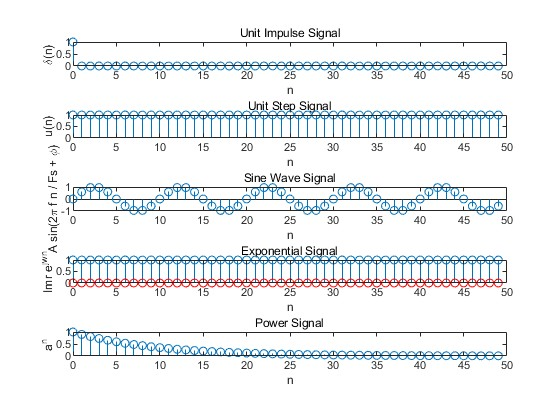
\includegraphics[width=0.8\linewidth]{images/1_Verify/five_signals.jpg}
\captionof{figure}{5种离散时间信号} 

\justifying

\subsubsection{讨论正弦序列、复指数序列的性质}
\begin{itemize}
    \item A.
    绘出信号$x(n) = e^{zn}$,当$Z = -\frac{1}{12} + j\frac{\pi}{6}$、$Z = \frac{1}{12} + j\frac{\pi}{6}$时、$Z = \frac{1}{12}$、$Z = 2 + j\frac{\pi}{6}$时的信号实部和虚部图;当$Z = j\frac{\pi}{6}$时呢?此时信号周期为多少?
\end{itemize}


首先,通过初始化参数,设置了样本数 \( N \) 和离散时间索引 \( n \),其中 \( N \) 表示样本数,\( n \) 表示从 \( 0 \) 到 \( N-1 \) 的离散时间索引。

然后,定义了不同的复数 \( Z \) 值,存储在 \( Z_{\text{values}} \) 数组中。这些复数值包含了不同的实部和虚部组合,用于生成不同的指数序列信号。

接下来,通过循环遍历每个 \( Z \) 值,生成相应的指数序列信号 \( x_n = \exp(Z \cdot n) \),并分别绘制其实部和虚部。每个信号的实部和虚部分别在一个新的图形中绘制,图形的标题和轴标签包含了对应的 \( Z \) 值。

最后,计算了特定参数 \( Z = j\pi/6 \) 对应的信号周期,并将结果输出到命令行窗口。

根据上述描述,可以得到以下代码:
\begin{lstlisting}
    % 初始化参数
N = 50; % 样本数
n = 0:N-1; % 离散时间索引

% 定义不同的 Z 值
Z_values = [-1/12 + 1j*pi/6, 1/12 + 1j*pi/6, 1/12, 2 + 1j*pi/6, 1j*pi/6];

% 分别计算和绘制每个 Z 值对应的信号
for k = 1:length(Z_values)
    Z = Z_values(k);
    x_n = exp(Z * n); % 生成信号

    % 绘制信号的实部
    figure;
    subplot(2, 1, 1);
    stem(n, real(x_n));
    title(['信号的实部,Z = ', num2str(real(Z)), ' + ', num2str(imag(Z)), 'j']);
    xlabel('n');
    ylabel('Re{x[n]}');

    % 绘制信号的虚部
    subplot(2, 1, 2);
    stem(n, imag(x_n));
    title(['信号的虚部,Z = ', num2str(real(Z)), ' + ', num2str(imag(Z)), 'j']);
    xlabel('n');
    ylabel('Im{x[n]}');
end

% 计算当 Z = j*pi/6 时的周期
Z_periodic = 1j*pi/6;
period = 2*pi / abs(imag(Z_periodic)); % 信号的周期

% 输出周期
disp(['当 Z = ', num2str(imag(Z_periodic)), 'j 时,信号的周期为: ', num2str(period)]);

\end{lstlisting}

得到的结果如下:
\begin{figure}[htbp]
    \centering
    \begin{minipage}[b]{0.48\textwidth}
        \centering
        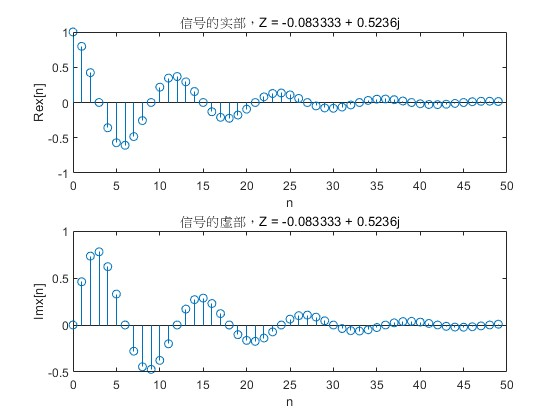
\includegraphics[width=\linewidth]{images/1_Verify/questionA_1.jpg}
        \caption{正弦序列、复指数序列性质1}
    \end{minipage}
    \hfill
    \begin{minipage}[b]{0.48\textwidth}
        \centering
        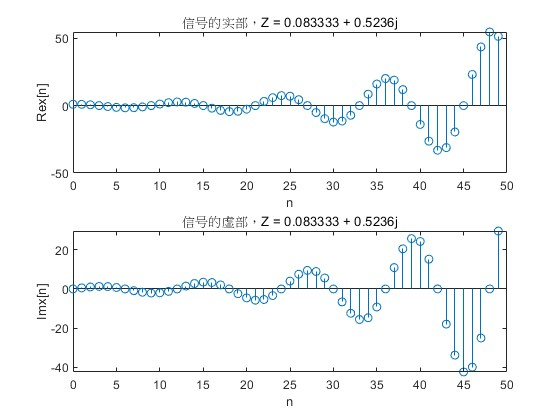
\includegraphics[width=\linewidth]{images/1_Verify/questionA_2.jpg}
        \caption{正弦序列、复指数序列性质2}
    \end{minipage}
\end{figure}

\begin{figure}[htbp]
    \centering
    \begin{minipage}[b]{0.48\textwidth}
        \centering
        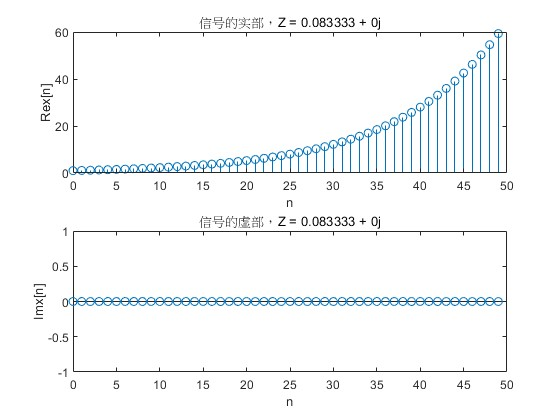
\includegraphics[width=\linewidth]{images/1_Verify/questionA_3.jpg}
        \caption{正弦序列、复指数序列性质3}
    \end{minipage}
    \hfill
    \begin{minipage}[b]{0.48\textwidth}
        \centering
        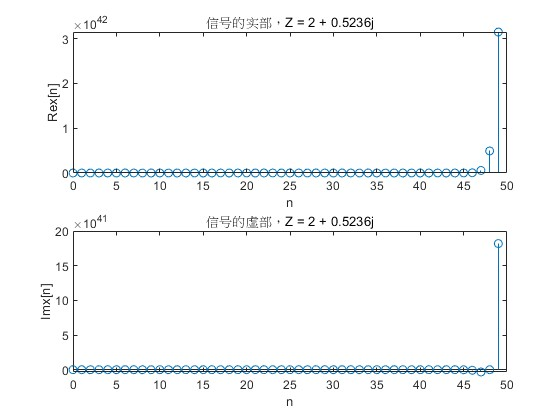
\includegraphics[width=\linewidth]{images/1_Verify/questionA_4.jpg}
        \caption{正弦序列、复指数序列性质4}
    \end{minipage}
\end{figure}

\centering 
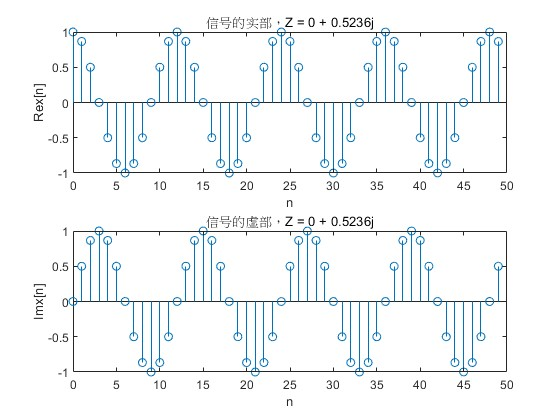
\includegraphics[width=0.6\linewidth]{images/1_Verify/questionA_5.jpg}
\captionof{figure}{正弦序列、复指数序列性质5} 

\justifying

\begin{itemize}
    \item B.
    绘出信号$x(n) = 1.5 \sin(2\pi \cdot 0.17n)$ 的频率是多少?周期是多少?产生一个数字频率为
0.9的正弦序列,并显示该信号,说明其周期。

\end{itemize}

首先,通过设定参数,设置了样本数 \( N \) 和离散时间索引 \( n \),以确保足够多的样本以显示信号的周期性。

然后,生成并绘制了一个离散时间正弦信号 \( x[n] = 1.5 \sin(2\pi \times 0.1n) \),其中幅值为 \(1.5\),频率为 \(0.1\),并将其显示在图形中。

接着,计算并显示了该信号的数字频率和周期,其中数字频率 \(f\) 的计算公式为 \( f = \frac{1}{T} \),其中 \(T\) 表示周期。

接下来,产生并绘制了一个具有不同数字频率 \(0.9\) 的正弦序列,并将其显示在图形中。

最后,计算并显示了新序列的周期 \(T2\),以便进一步分析新序列的周期性。

根据上述描述,可以得到以下代码:

\begin{lstlisting}
% 参数设定
N = 100; % 样本数,取足够多的样本以显示信号的周期性
n = 0:N-1; % 离散时间索引

% 绘制信号 x[n] = 1.5sin(2pi*0.1n)
x_n = 1.5 * sin(2 * pi * 0.1 * n);
\begin{figure}[htbp]
\centering
\begin{minipage}[b]{0.6\textwidth}
\centering
\includegraphics[width=\linewidth]{plot_1.jpg}
\caption{离散时间正弦信号 $x[n] = 1.5\sin(2\pi \times 0.1n)$}
\end{minipage}

% 信号的数字频率和周期
f = 0.1; % 数字频率
T = 1 / f; % 周期,样本数
\end{figure}

\begin{figure}[htbp]
\centering
\begin{minipage}[b]{0.6\textwidth}
\centering
\includegraphics[width=\linewidth]{plot_2.jpg}
\caption{数字频率为 $0.9$ 的正弦序列}
\end{minipage}

% 计算并显示新序列的周期
T2 = 1 / f2; % 周期,样本数
\end{figure}

\end{lstlisting}

得到的结果如下:
\begin{figure}[htbp]
    \centering
    \begin{minipage}[b]{0.48\textwidth}
        \centering
        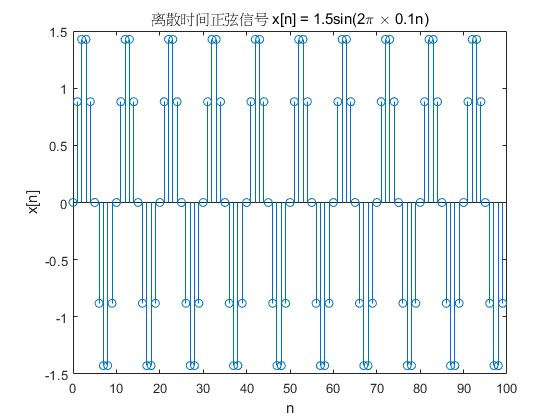
\includegraphics[width=\linewidth]{images/1_Verify/questionB_1.jpg}
        \caption{正弦序列、复指数序列性质6}
    \end{minipage}
    \hfill
    \begin{minipage}[b]{0.48\textwidth}
        \centering
        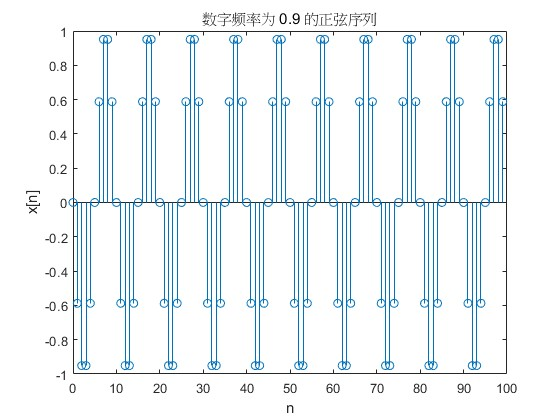
\includegraphics[width=\linewidth]{images/1_Verify/questionB_2.jpg}
        \caption{正弦序列、复指数序列性质7}
    \end{minipage}
    
\end{figure}


\subsubsection{学习方波、锯齿波和sinc函数并绘图}
首先,通过设定参数,设置了样本数 \( N \) 和离散时间索引 \( n \),以确保有足够的样本数来绘制信号。

然后,分别生成方波信号、锯齿波信号和sinc函数信号,并将它们存储在变量中。

接下来,使用 `subplot` 函数将三种信号分别绘制在三个子图中:
\begin{itemize}
    \item 第一个子图绘制了方波信号,标题为“离散时间方波信号”;
    \item 第二个子图绘制了锯齿波信号,标题为“离散时间锯齿波信号”;
    \item 第三个子图绘制了sinc函数信号,标题为“离散时间sinc函数信号”。
\end{itemize}

每个子图都有相应的轴标签来表示时间索引 \( n \) 和信号的幅值。

最后,使用 `figure` 函数显示所有的子图。

根据上述描述,可以得到以下代码:
\begin{lstlisting}
% 参数设定
N = 100; % 样本数,可以根据需要修改
n = 0:N-1; % 离散时间索引

% 生成方波信号
square_wave = square(2 * pi * 0.05 * n);

% 生成锯齿波信号
sawtooth_wave = sawtooth(2 * pi * 0.05 * n);

% 生成sinc函数信号
sinc_wave = sinc(n - N/2);

% 绘制方波信号
figure;
subplot(3, 1, 1);
stem(n, square_wave);
title('离散时间方波信号');
xlabel('n');
ylabel('Amplitude');

% 绘制锯齿波信号
subplot(3, 1, 2);
stem(n, sawtooth_wave);
title('离散时间锯齿波信号');
xlabel('n');
ylabel('Amplitude');

% 绘制sinc函数信号
subplot(3, 1, 3);
stem(n - N/2, sinc_wave);
title('离散时间sinc函数信号');
xlabel('n');
ylabel('Amplitude');

% 显示所有图形
figure;

\end{lstlisting}

可以得到以下结果:

\centering 
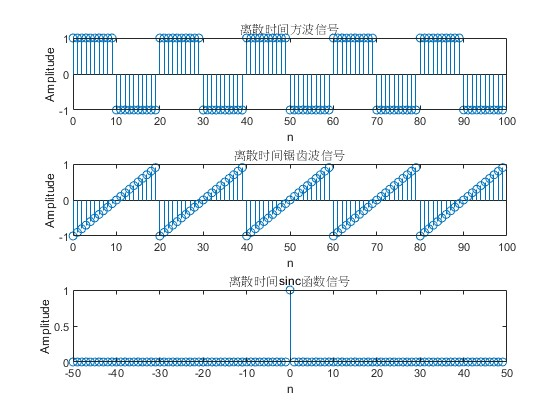
\includegraphics[width=0.6\linewidth]{images/1_Verify/question3.jpg}
\captionof{figure}{方波、锯齿波和sinc函数绘图} 

\justifying

\subsubsection{熟悉利用函数$y = filter(p,d,x)$实现差分方程的仿真}
首先,定义了滤波器的系数 $p$ 和 $d$。在这个示例中,假定滤波器的分子系数为 $[0.5, 0.5]$,分母系数为 $1$。

接着,生成了一个示例信号 $x$。这个信号是一个频率为 $0.05$ 的余弦信号,加上了服从标准正态分布的随机噪声,长度为 $N$。

然后,通过调用 \texttt{filter(p, d, x)} 函数,将定义的滤波器应用到示例信号 $x$ 上,得到滤波后的信号 $y$。

最后,使用 \texttt{subplot} 函数将原始信号和滤波后的信号分别绘制在两个子图中,以便比较它们的变化。原始信号绘制在第一个子图中,标题为“原始信号”;滤波后的信号绘制在第二个子图中,标题为“滤波后的信号”。

根据上述描述,可以得到以下matlab代码:
\begin{lstlisting}
% 滤波器系数,需要根据具体要求来定义
p = [0.5 0.5]; % 假定的滤波器分子系数
d = 1; % 假定的滤波器分母系数

% 生成一个示例信号
N = 100; % 信号长度
x = cos(2 * pi * 0.05 * (0:N-1)) + 0.5 * randn(1, N); % 一个频率的余弦信号加上噪声

% 应用滤波器
y = filter(p, d, x);

% 绘制原始信号和滤波后的信号
figure;
subplot(2, 1, 1);
plot(x);
title('原始信号');

subplot(2, 1, 2);
plot(y);
title('滤波后的信号');

\end{lstlisting}

得到的结果如下:

\centering 
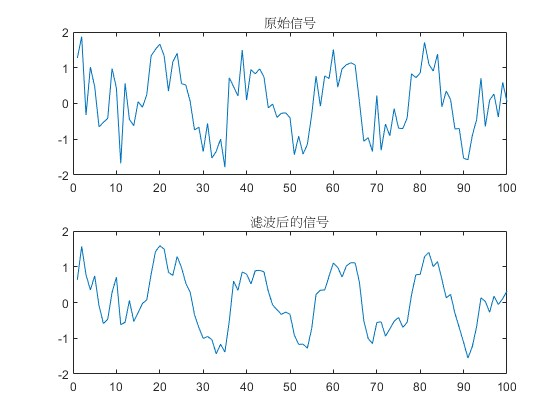
\includegraphics[width=0.6\linewidth]{images/1_Verify/preview1.jpg}
\captionof{figure}{函数$y = filter(p,d,x)$实现差分方程的仿真} 
\justifying

\subsubsection{熟悉用函数$y = conv(x,h)$计算卷积}
题目中使用 MATLAB 中的 \texttt{impz} 函数生成单位脉冲响应,并通过 \texttt{conv} 函数对信号和单位脉冲响应进行卷积。

首先,定义了示例的滤波器系数 $p$ 和 $d$,分别表示滤波器的分子系数和分母系数。在这个示例中,滤波器的分子系数为 $[1, -0.5]$,分母系数为 $[1, 0.5]$。

接着,通过调用 \texttt{impz(p, d, N)} 函数,生成了长度为 $N$ 的单位脉冲响应 $h[n]$。

然后,生成了一个示例信号 $x[n]$,这里使用一个长度为 $N$ 的全1序列来模拟。

接下来,通过 \texttt{conv} 函数对信号 $x[n]$ 和单位脉冲响应 $h[n]$ 进行卷积操作,得到卷积结果 $y[n]$。

最后,使用 \texttt{subplot} 函数将单位脉冲响应和卷积结果分别绘制在两个子图中,以便比较它们的形态特征。单位脉冲响应绘制在第一个子图中,标题为“单位脉冲响应 $h[n]$”;卷积结果绘制在第二个子图中,标题为“信号 $x[n]$ 和 $h[n]$ 的卷积结果 $y[n]$”。

\begin{lstlisting}
% 滤波器系数
p = [1, -0.5]; % 示例滤波器分子系数
d = [1, 0.5];  % 示例滤波器分母系数
N = 10;        % 单位脉冲响应的长度

% 生成单位脉冲响应
h = impz(p, d, N);

% 生成信号 x[n]
x = ones(1, N); % 示例信号,这里我们只是用一个长度为 N 的全1序列来模拟

% 对信号 x[n] 和单位脉冲响应 h[n] 进行卷积
y = conv(x, h);

% 绘制单位脉冲响应
figure;
subplot(2, 1, 1);
stem(h);
title('单位脉冲响应 h[n]');

% 绘制卷积结果
subplot(2, 1, 2);
stem(y);
title('信号 x[n] 和 h[n] 的卷积结果 y[n]');
xlabel('n');
ylabel('Amplitude');

\end{lstlisting}

得到的结果如下:

\centering 
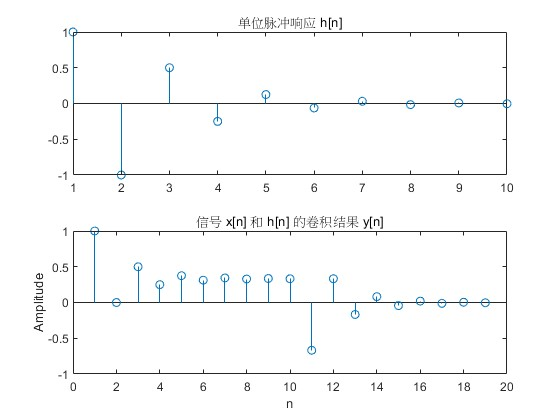
\includegraphics[width=0.6\linewidth]{images/1_Verify/preview2.jpg}
\captionof{figure}{函数$y = conv(x,h)$计算卷积} 
\justifying

\subsubsection{熟悉用filter函数计算卷积}
\begin{itemize}
    \item 以下程序中分别使用 \texttt{conv} 和 \texttt{filter} 函数计算 \( h \) 和 \( x \) 的卷积 \( y \) 和 \( y_1 \),运行程序,并分析 \( y \) 和 \( y_1 \) 是否有差别。为什么要使用 \( x[n] \) 补零后的 \( x_1 \) 来产生 \( y_1 \);具体分析当 \( h[n] \) 有 \( i \) 个值,\( x[n] \) 有 \( j \) 个值,使用 \texttt{filter} 完成卷积功能,需要如何补零?

\begin{lstlisting}
% Program P2_7
clf;
h = [3 2 1 -2 1 0 -4 0 3]; %impulse response
x = [1 -2 3 -4 3 2 1]; %input sequence
y = conv(h,x);
n = 0:14;
subplot(2,1,1);
stem(n,y);
xlabel('Time index n'); ylabel('Amplitude');
title('Output Obtained by Convolution'); grid;
x1 = [x zeros(1,8)];
y1 = filter(h,1,x1);
subplot(2,1,2);
stem(n,y1);
xlabel('Time index n'); ylabel('Amplitude');
title('Output Generated by Filtering'); grid;
\end{lstlisting}
运行上述代码,可以得到以下结果:

\centering 
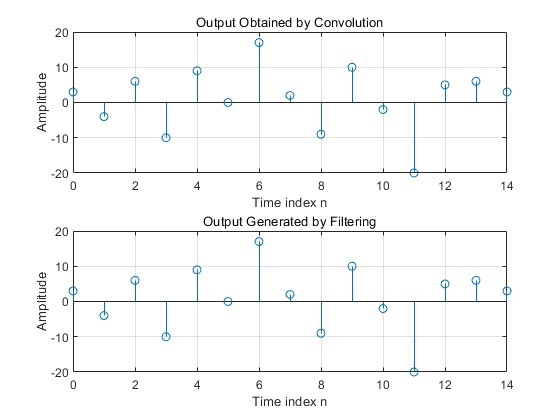
\includegraphics[width=0.6\linewidth]{images/1_Verify/exp1.jpg}
\captionof{figure}{filter函数计算卷积结果} 
\justifying

以上程序使用了 \texttt{conv} 函数和 \texttt{filter} 函数来计算序列 \( h \) 和 \( x \) 的卷积,生成了 \( y \) 和 \( y_1 \)。根据程序,我们可以分析两种方法的结果是否有差异,以及为什么需要在使用 \texttt{filter} 函数时对 \( x[n] \) 进行补零。

\textbf{卷积和滤波的差异}:
\begin{itemize}
    \item \texttt{conv} 函数计算两个序列的完整卷积。这意味着,如果 \( h[n] \) 有 \( i \) 个值,\( x[n] \) 有 \( j \) 个值,那么 \texttt{conv(h, x)} 的结果 \( y \) 将会有 \( i+j-1 \) 个值。
    \item \texttt{filter} 函数设计为一个实时滤波器,它应用滤波器的系数对输入信号 \( x[n] \) 进行滤波。在不补零的情况下,使用 \texttt{filter(h, 1, x)} 时,输出的长度与输入 \( x[n] \) 的长度相同。
\end{itemize}

因为 \texttt{conv} 和 \texttt{filter} 的操作定义不同,所以 \texttt{filter} 在处理信号时不会自动扩展输出的长度。为了使 \texttt{filter} 函数的输出与 \texttt{conv} 的输出长度相同,需要对输入信号 \( x[n] \) 进行补零。

\textbf{为什么要补零}:
\begin{itemize}
    \item 补零是为了获得与卷积等长的输出,从而可以比较 \texttt{conv} 和 \texttt{filter} 的结果。
    \item 当使用 \texttt{filter} 函数时,补零还有一个目的,那就是模拟卷积操作中输入序列和单位脉冲响应两端的“尾部”相乘的效果。
\end{itemize}

\textbf{具体补零的方法}:
\begin{itemize}
    \item 如果 \( h[n] \) 有 \( i \) 个值,\( x[n] \) 有 \( j \) 个值,那么需要在 \( x[n] \) 后面补零,补 \( i-1 \) 个零,以确保 \texttt{filter} 的输出具有 \( i+j-1 \) 个值,与 \texttt{conv} 的结果长度相匹配。
\end{itemize}

根据程序,我们可以这样分析:

\( h[n] \) 有 9 个值,\( x[n] \) 有 7 个值,那么 \texttt{conv(h, x)} 生成的 \( y \) 将会有 \( 9+7-1=15 \) 个值。为了使 \texttt{filter} 产生同样长度的输出,我们需要在 \( x[n] \) 后面补 \( 9-1=8 \) 个零,这就是为什么 \texttt{x1 = [x zeros(1,8)]} 的原因。

运行程序并观察 \( y \) 和 \( y_1 \) 的结果,我们可以发现,在补零后,\texttt{filter} 生成的输出 \( y_1 \) 在长度上与 \texttt{conv} 生成的 \( y \) 相同。如果在不补零的情况下使用 \texttt{filter},其结果将会在达到 \( x[n] \) 末端时结束,这样就不能完全展示 \( h[n] \) 对 \( x[n] \) 的完整卷积影响。补零后,\texttt{filter} 产生的输出包含了卷积的所有非零部分,更准确地反映了 \( h[n] \) 和 \( x[n] \) 卷积的实际结果。

\end{itemize}


\subsubsection{使用不同函数求解系统冲激与阶跃响应}
编制程序求解下列两个系统的单位冲激响应和阶跃响应,并绘出其图形。要求分别用 filter、
conv、impz 三种函数完成。
\begin{itemize}
    \item system A:$y[n] + 0.75y[n-1] + 0.125y[n-2] = x[n] - x[n-1]$
    \item system B:$y[n] = 0.25\{x[n-1] + x[n-2] +x[n -3] + x[n-4]\}$
\end{itemize}

\textbf{system A:}
\begin{itemize}
    \item 首先,定义了一个系统的分子系数 \texttt{num} 和分母系数 \texttt{den}。
    \item 接下来,定义了序列的长度 \texttt{len1},以及离散时间索引 \texttt{n} 和 \texttt{n1}。
    \item 创建了单位冲激序列 \texttt{xn}(一个脉冲后跟一系列零)和阶跃序列 \texttt{yn}(一系列单位幅度的1)。
    \item 使用 \texttt{filter} 函数计算了滤波器的单位冲激响应 \texttt{hn1} 和阶跃响应 \texttt{sn1},并绘制了相应的图形。
    \item 使用 \texttt{conv} 函数计算了滤波器的单位冲激响应 \texttt{hn2} 和阶跃响应 \texttt{sn2},并绘制了相应的图形。
    \item 使用 \texttt{impz} 函数计算了单位冲激响应 \texttt{hn3},并使用 \texttt{conv} 函数计算了阶跃响应 \texttt{sn3},并绘制了相应的图形。
\end{itemize}

代码通过绘制三种方法计算的单位冲激响应和阶跃响应的图形,来比较它们的结果。

\begin{lstlisting}
num=[1,-1];
den=[1,0.75,0.125];
len1=15;
n=0:len1;
n1=0:2*len1;

xn=[1,zeros(1,15)];
yn=ones(1,16);
hn1=filter(num,den,xn);
sn1=filter(num,den,yn);
subplot(2,3,1);
stem(n,hn1);
title("单位冲激响应(filter)");
xlabel("n");ylabel("hn");
subplot(2,3,4);
stem(n,sn1);
title("阶跃响应(filter)");
xlabel("n");ylabel("sn");

hn2=conv(xn,impz(num,den,n));
sn2=conv(yn,impz(num,den,n));
subplot(2,3,2);
stem(n,hn1);
title("单位冲激响应(conv)");
xlabel("n");ylabel("hn");
subplot(2,3,5);
stem(n,sn1);
title("阶跃响应(conv)");
xlabel("n");ylabel("sn");

hn3=impz(num,den,n);
sn3=conv(yn,hn3);
subplot(2,3,3);
stem(n,hn3);
title("单位冲激响应(impz)");
xlabel("n");ylabel("hn");
subplot(2,3,6);
stem(n1,sn3)
title("阶跃响应(impz)");
xlabel("n");ylabel("sn");
axis([0,len1,-0.8, 1]);
\end{lstlisting}

得到的结果如下:

\centering 
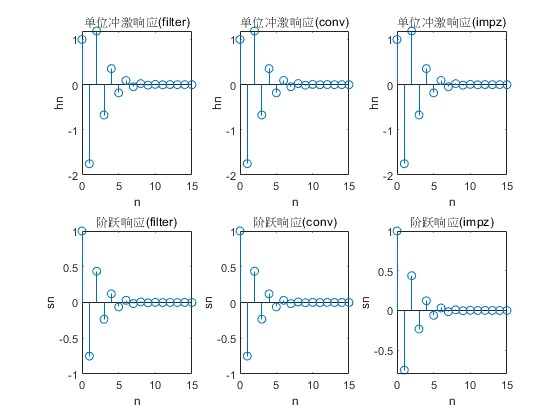
\includegraphics[width=0.8\linewidth]{images/1_Verify/exp2_1.jpg}
\captionof{figure}{单位冲激响应和阶跃响应结果} 
\justifying

现在进行验证:

$y[n] + 0.75y[n-1] + 0.125y[n-2] = x[n] - x[n-1]$

\begin{itemize}
    \item 传递函数 \( H(Z) = \frac{Y(Z)}{X(Z)} = \frac{6}{1 + 0.5Z^{-1}} - \frac{5}{1 + 0.25Z^{-1}} \)
    \item 单位冲激响应 \( h[n] = 6 \cdot (-0.5)^n \cdot u[n] - 5 \cdot (-0.25)^n \cdot u[n] \)
    \item 单位阶跃响应 \( y[n] = h[n] \cdot u[n] = 4 \cdot (-0.25)^{n+1} - 4 \cdot (-0.5)^{n+1} \)
\end{itemize}

\centering 
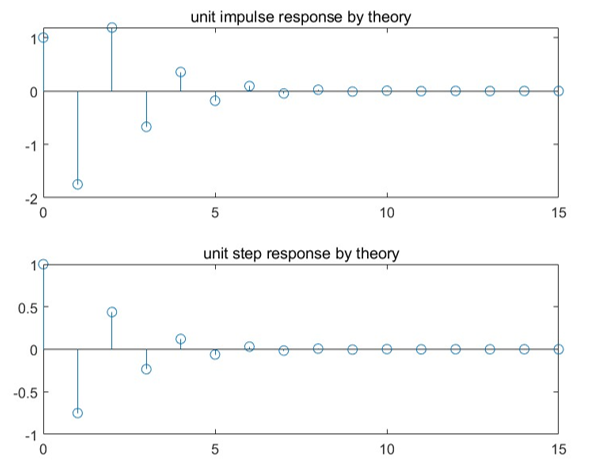
\includegraphics[width=0.6\linewidth]{images/1_Verify/theory1.png}
\captionof{figure}{系统A理论计算结果} 
\justifying

可见理论计算结果与代码运行结果一致。

\textbf{system B:}
\begin{itemize}
    \item 首先,定义了系统的传递函数的分子系数 \texttt{num} 和分母系数 \texttt{den}。
    \item 接下来,定义了序列的长度 \texttt{len1},以及离散时间索引 \texttt{n} 和 \texttt{n1}。
    \item 创建了单位冲激序列 \texttt{xn}(一个脉冲后跟一系列零)和阶跃序列 \texttt{yn}(一系列单位幅度的1)。
    \item 使用 \texttt{filter} 函数计算了系统的单位冲激响应 \texttt{hn1} 和阶跃响应 \texttt{sn1},并绘制了相应的图形。
    \item 使用 \texttt{conv} 函数计算了系统的单位冲激响应 \texttt{hn2} 和阶跃响应 \texttt{sn2},并绘制了相应的图形。
    \item 使用 \texttt{impz} 函数计算了系统的单位冲激响应 \texttt{hn3},并使用 \texttt{conv} 函数计算了阶跃响应 \texttt{sn3},并绘制了相应的图形。
\end{itemize}

通过绘制三种方法计算的单位冲激响应和阶跃响应的图形,可以比较它们的结果。

\begin{lstlisting}
num=[0,0.25,0.25,0.25,0.25];
den=1;
len1=30;
n=0:len1;
n1=0:2*len1;

xn=[1,zeros(1,len1)];
yn=ones(1,len1+1);
hn1=filter(num,den,xn);
sn1=filter(num,den,yn);
subplot(2,3,1);
stem(n,hn1);
title("单位冲激响应(filter)");xlabel("n");ylabel("hn");
subplot(2,3,4);
stem(n,sn1);
title("阶跃响应(filter)");xlabel("n");ylabel("sn");

hn2=conv(xn,impz(num,den,n));
sn2=conv(yn,impz(num,den,n));
subplot(2,3,2);
stem(n,hn1);
title("单位冲激响应(conv)");xlabel("n");ylabel("hn");
subplot(2,3,5);
stem(n,sn1);
title("阶跃响应(conv)");xlabel("n");ylabel("sn");

hn3=impz(num,den,n);
sn3=conv(yn,hn3);
subplot(2,3,3);
stem(n,hn3);
title("单位冲激响应(impz)");xlabel("n");ylabel("hn");
subplot(2,3,6);
stem(n1,sn3)
title("阶跃响应(impz)");xlabel("n");ylabel("sn");
axis([0,len1,0,1]);

\end{lstlisting}

得到的结果如下:

\centering 
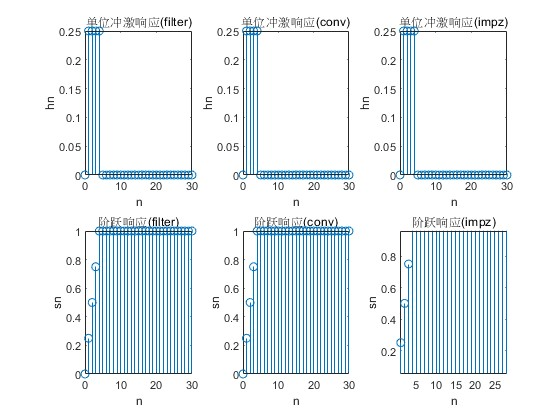
\includegraphics[width=0.8\linewidth]{images/1_Verify/exp2_2.jpg}
\captionof{figure}{单位冲激响应和阶跃响应结果} 
\justifying

现在进行验证:

$y[n] = 0.25\{x[n-1] + x[n-2] +x[n -3] + x[n-4]\}$

\begin{itemize}
    \item 单位冲激响应:\[h[n]=0.25 \delta[n-1]+0.25 \delta[n-2]+0.25 \delta[n-3]+0.25 \delta[n-4]\]
    \item 单位阶跃响应:\[y[n]=h[n]*u[n]=0.25u[n-1]+0.5u[n-2]+0.75u[n-3]+u[n-4]\]

\end{itemize}

这样的结果可以表示系统对于单位冲激和单位阶跃的响应。

\centering 
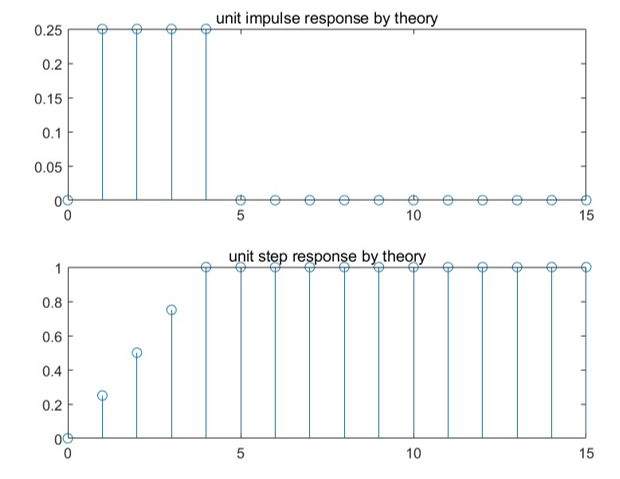
\includegraphics[width=0.6\linewidth]{images/1_Verify/theory2.png}
\captionof{figure}{系统B理论计算结果} 
\justifying

可见理论计算结果与代码运行结果一致。

\newpage
\section{应用性实验}
\subsection{实验目的}
\begin{itemize}
    \item 每人录制一段自己的拼音字母“a、o、e”四个声调、和任意一句话的声音(注意采样率)
    \item 利用自相关法或者其他方法实现声音信号的基音周期估计,观察不同字母、声调的基音变化 
    \item 编写一个频率可调、声音大小可调的函数,实现能产生20Hz到20kHz的响度可调的单频声音信号, 以测试各自的听觉范围

\end{itemize}
\subsection{实验原理}
\subsubsection{语音基因周期估计}
\begin{itemize}
    \item 自相关法:

    自相关法是一种常用的语音信号处理方法,用于估计基音周期。其原理基于声音信号的周期性特征。在语音中,周期性的声音通常是由声带的振动引起的,这种振动产生了声音信号中的周期性重复模式。自相关法通过计算信号与其自身的延迟版本之间的相关性,来寻找这种周期性重复的模式。具体而言,自相关函数表示了信号与其在时间轴上向后延迟一定时间后的版本之间的相似程度。在语音信号中,基音周期导致了自相关函数的周期性峰值。通过寻找这些峰值,我们可以得到声音信号中基音周期的估计值。\cite{atkinson1979pitch}

    \item 基音周期:

    基音周期是语音信号中的一个重要参数,它决定了声音的音调和音高。在声音合成和语音分析中,基音周期通常用来描述声音的基频特征。基音周期表示了声带振动的周期性,即声带在一次完整振动周期内完成的时间。基音周期越短,声音的音调越高,反之亦然。因此,基音周期是语音合成中一个关键的参数,能够影响合成声音的音质和自然度。

    \item 基音周期估计:
    
    基音周期估计是通过分析语音信号的自相关函数来确定声音中的基音周期。自相关函数反映了信号的周期性重复模式,而语音信号的基音周期正是导致这种重复的主要原因。基音周期估计的目标是通过计算自相关函数的峰值来确定基音周期的位置。在实践中,我们通常会对自相关函数进行归一化处理,以提高基音周期估计的准确性和稳定性。

    \item 声调的基音变化:
    
    声调是语言中的一个重要语音特征,指的是声音的音高变化。不同声调下的语音信号具有不同的基音周期,这导致了声音在音高上的变化。通过观察不同声调下的基音周期变化,我们可以了解声音在不同语境下的音高表现。例如,在普通话中,声调的不同会导致同一个音节的基音周期有所不同,从而产生不同的音调效果。因此,观察声调的基音变化有助于我们理解语音信号的基本特征和语言表达方式。


    
\end{itemize}
\subsubsection{听力测试信号发生器}
这个实验的目标是编写一个函数,能够产生频率可调、声音大小可调的单频声音信号,其频率范围从20Hz到20kHz,以便测试听众的听觉范围。下面是实验原理的详细解释:
\begin{itemize}
    \item 频率可调:

       实现频率可调的单频声音信号,可以利用正弦波函数来生成。正弦波的频率由以下公式给出:
   
   \[ f = \frac{n}{T} \]

   其中,\( f \) 是频率, \( T \) 是周期, \( n \) 是正弦波的周期数。因此,我们可以通过调整正弦波的周期数来实现频率的可调性。将周期数与所需的频率相对应,可以在20Hz到20kHz的范围内产生不同频率的正弦波声音。

   \item 声音大小可调:
   
      实现声音大小可调需要对正弦波进行幅度调节。通常,音频信号的幅度由其振幅决定。通过调整正弦波的振幅,我们可以改变声音的大小或响度。在实验中,可以提供一个参数来控制正弦波的振幅,使用户可以调节声音的大小。通过提供这样的参数,用户可以在测试听觉范围时自由地调节声音的响度,以满足个人的需求和偏好。

\end{itemize}

通过控制正弦波的周期数和振幅,我们可以编写一个函数来生成频率可调、声音大小可调的单频声音信号。这样的函数将允许用户在20Hz到20kHz的范围内产生不同频率和不同响度的声音,以测试其听觉范围和敏感度。

\subsection{实验内容}
\subsubsection{使用自相关法进行语音基音周期估计}
根据实验要求,可以将任务分成三个部分:
\begin{itemize}
    \item 加载音频文件:
使用 \texttt{audioread} 函数加载了四个音频文件:分别是表示拼音字母 "a"、"e"、"o" 的音频文件,以及包含一句话的音频文件。
对于每个音频文件,分别存储了音频信号和采样率。

    \item 基音周期估计:
    调用了名为 \texttt{estimate\_pitch} 的函数对每个音频文件进行基音周期的估计。
\texttt{estimate\_pitch} 函数的输入是音频信号和对应的采样率,输出是基音周期的估计值。
对于每个音频文件,获取了基音周期的估计值,分别存储在 \texttt{a\_pitch\_periods}、\texttt{e\_pitch\_periods}、\texttt{o\_pitch\_periods} 和 \texttt{sentence\_pitch\_periods} 中。

    \item 绘制基音周期的变化曲线:
    使用 \texttt{subplot} 函数创建了一个 4x1 的图形窗口,用于分别绘制每个音频文件的基音周期变化曲线。
在每个子图中,调用 \texttt{plot} 函数绘制了基音周期随时间变化的曲线。
每个子图的横轴表示帧索引,纵轴表示基音周期(以采样点数为单位)。
\end{itemize}

根据上述描述,可以得到以下代码:
\begin{lstlisting}
% 主程序
% 加载音频文件
[a_signal, a_fs] = audioread('a.m4a');
[e_signal, e_fs] = audioread('e.m4a');
[o_signal, o_fs] = audioread('o.m4a');
[sentence_signal, sentence_fs] = audioread('sentence1.m4a');

% 对每个音频文件进行基音周期估计
a_pitch_periods = estimate_pitch(a_signal, a_fs);
e_pitch_periods = estimate_pitch(e_signal, e_fs);
o_pitch_periods = estimate_pitch(o_signal, o_fs);
sentence_pitch_periods = estimate_pitch(sentence_signal, sentence_fs);

% 绘制基音周期的变化曲线
figure;
subplot(4, 1, 1);
plot(a_pitch_periods);
title('Pitch Periods for "a"');
xlabel('Frame Index');
ylabel('Pitch Period (samples)');

subplot(4, 1, 2);
plot(e_pitch_periods);
title('Pitch Periods for "e"');
xlabel('Frame Index');
ylabel('Pitch Period (samples)');

subplot(4, 1, 3);
plot(o_pitch_periods);
title('Pitch Periods for "o"');
xlabel('Frame Index');
ylabel('Pitch Period (samples)');

subplot(4, 1, 4);
plot(sentence_pitch_periods);
title('Pitch Periods for Sentence');
xlabel('Frame Index');
ylabel('Pitch Period (samples)');
\end{lstlisting}

其中\texttt{estimate\_pitch}函数代码思路如下:
以下代码实现了基音周期的估计函数 \texttt{estimate\_pitch}。下面是它的主要步骤:

\begin{itemize}
    \item \textbf{参数设置}:根据采样率 \texttt{fs},确定帧长和帧移的采样点数,通常为 20 毫秒一帧,帧移 10 毫秒。
    
    \item \textbf{分帧处理}:将输入信号 \texttt{signal} 进行分帧处理,得到一系列重叠的帧。
    
    \item \textbf{初始化基音周期数组}:创建一个数组 \texttt{pitch\_periods} 用于存储每个帧的基音周期估计值。
    
    \item \textbf{基音周期估计}:对每一帧进行基音周期的估计。
    \begin{itemize}
        \item 首先,根据帧的索引计算该帧在信号中的起始采样点和结束采样点。
        \item 然后,提取该帧的信号。
        \item 计算帧信号的自相关函数,即信号与其自身的相关性。
        \item 在自相关函数中找到第一个局部极大值,将其位置作为基音周期的估计值。如果找不到局部极大值,则将基音周期估计值设为 \texttt{NaN}。
    \end{itemize}
    
    \item 返回基音周期数组 \texttt{pitch\_periods}。
\end{itemize}

这个函数主要利用自相关函数的性质,在自相关函数中找到局部极大值来估计基音周期。

\begin{lstlisting}
% 基音周期估计函数
function pitch_periods = estimate_pitch(signal, fs)
    % 参数设置
    frame_length = round(0.02 * fs);  % 20ms一帧
    frame_shift = round(0.01 * fs);   % 帧移10ms

    % 分帧处理
    num_samples = length(signal);
    num_frames = floor((num_samples - frame_length) / frame_shift) + 1;

    % 初始化基音周期数组
    pitch_periods = zeros(num_frames, 1);

    % 对每一帧进行基音周期估计
    for i = 1:num_frames
        start_sample = (i - 1) * frame_shift + 1;
        end_sample = start_sample + frame_length - 1;
        
        if end_sample > num_samples
            break;
        end
        
        frame = signal(start_sample:end_sample);
        
        % 计算自相关函数
        autocorr = xcorr(frame);
        autocorr = autocorr(frame_length:end);  % 取正向自相关函数部分

        % 找到第一个局部极大值,即为基音周期
        [~, locs] = findpeaks(autocorr, 'MinPeakHeight', max(autocorr) * 0.2);  % 设置阈值
        if isempty(locs)
            pitch_periods(i) = NaN;  % 找不到局部极大值,设为NaN
        else
            pitch_periods(i) = locs(1);  % 取第一个局部极大值位置作为周期
        end
    end
end
\end{lstlisting}

得到的实验结果如下图:

\centering 
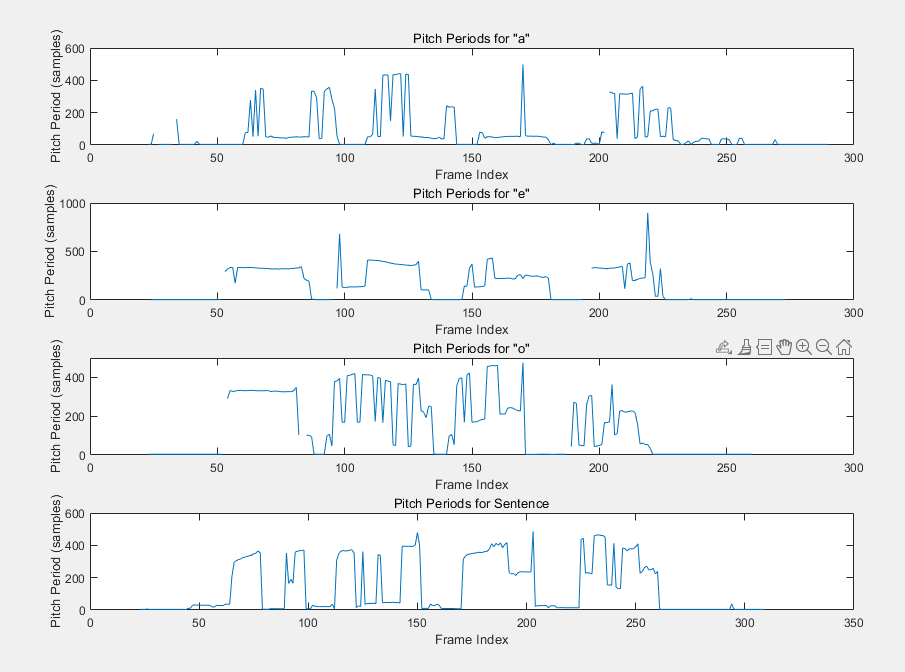
\includegraphics[width=0.8\linewidth]{images/1_Application/cycle.png}
\captionof{figure}{自相关法得到4个语音基音周期} 
\justifying

\subsubsection{使用倒谱法进行语音基音周期估计}
在本方法中,倒谱法的相关函数描述如下\cite{atal1974automatic}:

\begin{itemize}
    \item \textbf{参数设置}:
        \begin{itemize}
            \item \texttt{frame\_length}:每帧的采样点数,通常设置为一个固定的时间长度,这里是 20 毫秒。
            \item \texttt{frame\_shift}:帧之间的重叠长度,通常是帧长度的一半,这里是 10 毫秒。
            \item \texttt{fs}:采样率(每秒采样点数)。
        \end{itemize}
    
    \item \textbf{分帧处理}:
        \begin{itemize}
            \item 计算信号的总样本数 \texttt{num\_samples}。
            \item 根据帧长度和帧移计算出总帧数 \texttt{num\_frames}。
        \end{itemize}
    
    \item \textbf{初始化基音周期数组}:
        \begin{itemize}
            \item 创建一个大小为 \texttt{num\_frames} 的数组,用于存储每帧的基音周期。
        \end{itemize}
    
    \item \textbf{对每一帧进行基音周期估计}:
        \begin{itemize}
            \item 使用循环遍历每一帧。
            \item 计算当前帧的起始采样点和结束采样点。
            \item 截取当前帧的信号数据。
            \item 计算当前帧的倒谱(cepstrum)。
            \item 在倒谱中找到峰值,作为基音周期的估计值。
        \end{itemize}
\end{itemize}

根据以上描述,可以得到以下代码:
\begin{lstlisting}
function pitch_periods = daopu(signal, fs)
    % 参数设置
    frame_length = round(0.02 * fs);  % 20ms一帧
    frame_shift = round(0.01 * fs);   % 帧移10ms

    % 分帧处理
    num_samples = length(signal);
    num_frames = floor((num_samples - frame_length) / frame_shift) + 1;

    % 初始化基音周期数组
    pitch_periods = zeros(num_frames, 1);

    % 对每一帧进行基音周期估计
    for i = 1:num_frames
        start_sample = (i - 1) * frame_shift + 1;
        end_sample = start_sample + frame_length - 1;
        
        if end_sample > num_samples
            break;
        end
        
        frame = signal(start_sample:end_sample);
        
        % 计算倒谱
        cepstrum = ifft(log10(abs(fft(frame))));

        % 找到倒谱中的峰值,即为基音周期
        [~, locs] = findpeaks(cepstrum, 'MinPeakHeight', max(cepstrum) * 0.2);  % 设置阈值
        if isempty(locs)
            pitch_periods(i) = NaN;  % 找不到峰值,设为NaN
        else
            pitch_periods(i) = locs(1);  % 取第一个峰值位置作为周期
        end
    end
end

\end{lstlisting}

可以得到以下结果:
\centering 
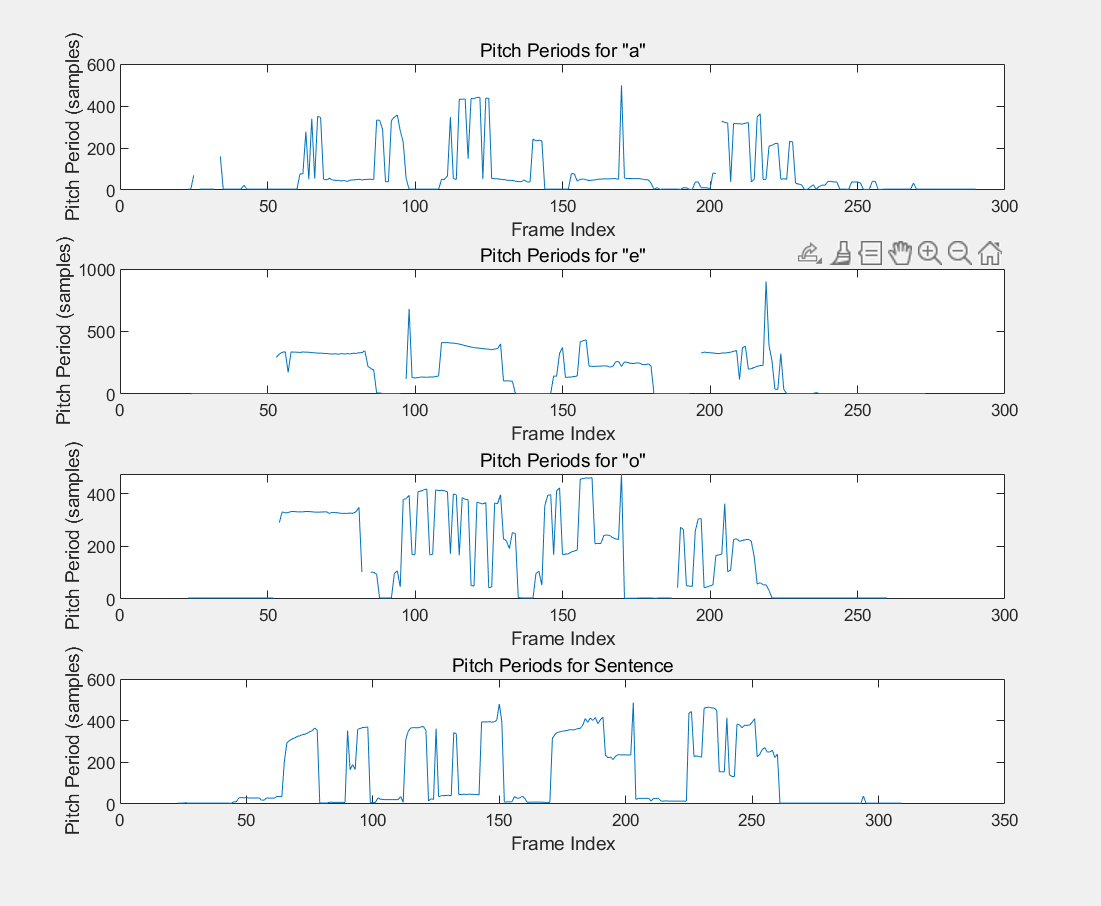
\includegraphics[width=0.8\linewidth]{images/1_Application/daopu.png}
\captionof{figure}{倒谱法得到4个语音基音周期} 
\justifying

经过分析,可以得到通过自相关法和倒谱法获得的a的四个声调的基音频率如下表:

\begin{table}[h]
\centering
\caption{a 四个音调的基音频率 (单位: Hz)}
\begin{tabular}{|c|c|c|c|c|}
\hline
\textbf{} & \textbf{第一声} & \textbf{第二声} & \textbf{第三声} & \textbf{第四声} \\ \hline
\textbf{自相关法} & 107 & 147 & 166 & 123 \\ \hline
\textbf{倒谱法} & 113 & 160 & 165 & 130 \\ \hline
\end{tabular}
\end{table}

通过自相关法和倒谱法获得的o的四个声调的基音频率如下表:

\begin{table}[h]
\centering
\caption{o 四个音调的基音频率 (单位: Hz)}
\begin{tabular}{|c|c|c|c|c|}
\hline
\textbf{} & \textbf{第一声} & \textbf{第二声} & \textbf{第三声} & \textbf{第四声} \\ \hline
\textbf{自相关法} & 106 & 136 & 134 & 96 \\ \hline
\textbf{倒谱法} & 107 & 139 & 138 & 100 \\ \hline
\end{tabular}
\end{table}

通过自相关法和倒谱法获得的e的四个声调的基音频率如下表:

\begin{table}[h]
\centering
\caption{e 四个音调的基音频率 (单位: Hz)}
\begin{tabular}{|c|c|c|c|c|}
\hline
\textbf{} & \textbf{第一声} & \textbf{第二声} & \textbf{第三声} & \textbf{第四声} \\ \hline
\textbf{自相关法} & 108 & 127 & 133 & 97 \\ \hline
\textbf{倒谱法} & 109 & 150 & 133 & 123 \\ \hline
\end{tabular}
\end{table}

通过自相关法和倒谱法获得的一句话的基音频率的基音频率大致在100Hz - 200Hz处。


\subsubsection{编写函数实现听力测试信号发生器}
实现听力测试信号发生器分成两个部分,其一是信号生成\texttt{hear\_test(f0, A)}函数,其二是用户交互GUI界面。

当使用\texttt{hear\_test(f0, A)}函数时:

\begin{itemize}
    \item \texttt{f0}:表示信号的频率。
    \item \texttt{A}:表示信号的振幅。
    \item 采样率:$8000 \, \text{Hz}$。
    \item 信号长度:$1$秒。
    \item 信号样本数:$N = 8000$个。
    \item 信号的时间轴:$n = 1, 2, \ldots, 8000$。
    \item 生成的信号$s(t)$:$s(t) = A \cdot \cos(2\pi f_0 \cdot t)$,其中$t$表示时间。
\end{itemize}

信号$s(t)$是一个正弦波信号,其频率由\texttt{f0}确定,振幅由\texttt{A}确定。

\texttt{hear\_test(f0, A)}函数代码如下:
\begin{lstlisting}
function s = hear_test(f0, A)
fs = 8000; 
N = fs*1;
n = 1:N;
s = A*cos(2*pi*f0*n/fs);
% subplot(2,1,1)
% plot(n,s)
sound(s,fs)


\end{lstlisting}

第二个部分是 GUI(图形用户界面)应用程序,它包含了一个窗口和一些控件,如文本框、按钮等。主要功能如下:

\begin{itemize}
    \item \texttt{gui} 函数是整个 GUI 应用程序的入口点,用于设置 GUI 的各种属性和事件处理函数。
    \item \texttt{gui\_OpeningFcn} 函数在 GUI 被打开时执行,用于初始化 GUI 界面。
    \item \texttt{gui\_OutputFcn} 函数定义了 GUI 的输出,通常是在 GUI 关闭时返回一些数据。
    \item \texttt{edit1} 和 \texttt{edit2} 是用于输入数字的文本框控件,分别用于输入信号的频率 (\texttt{f}) 和振幅 (\texttt{A})。
    \item \texttt{pushbutton1} 是一个按钮,当点击时会触发 \texttt{pushbutton1\_Callback} 函数。
    \item \texttt{pushbutton1\_Callback} 函数被触发时,它会从文本框 \texttt{edit1} 和 \texttt{edit2} 中获取用户输入的频率 (\texttt{f}) 和振幅 (\texttt{A}),然后调用 \texttt{hear\_test} 函数,并将这些参数传递给它。
\end{itemize}

这个 GUI 应用程序的主要功能是根据用户输入的频率和振幅生成一个正弦波信号,并播放该信号。

\begin{lstlisting}
function varargout = gui(varargin)
% GUI MATLAB code for gui.fig
gui_Singleton = 1;
gui_State = struct('gui_Name',       mfilename, ...
                   'gui_Singleton',  gui_Singleton, ...
                   'gui_OpeningFcn', @gui_OpeningFcn, ...
                   'gui_OutputFcn',  @gui_OutputFcn, ...
                   'gui_LayoutFcn',  [] , ...
                   'gui_Callback',   []);
if nargin && ischar(varargin{1})
    gui_State.gui_Callback = str2func(varargin{1});
end

if nargout
    [varargout{1:nargout}] = gui_mainfcn(gui_State, varargin{:});
else
    gui_mainfcn(gui_State, varargin{:});
end
% End initialization code - DO NOT EDIT


% --- Executes just before gui is made visible.
function gui_OpeningFcn(hObject, eventdata, handles, varargin)
% This function has no output args, see OutputFcn.
% hObject    handle to figure
% eventdata  reserved - to be defined in a future version of MATLAB
% handles    structure with handles and user data (see GUIDATA)
% varargin   command line arguments to gui (see VARARGIN)

% Choose default command line output for gui
handles.output = hObject;

% Update handles structure
guidata(hObject, handles);

% UIWAIT makes gui wait for user response (see UIRESUME)
% uiwait(handles.figure1);


% --- Outputs from this function are returned to the command line.
function varargout = gui_OutputFcn(hObject, eventdata, handles) 
% varargout  cell array for returning output args (see VARARGOUT);
% hObject    handle to figure
% eventdata  reserved - to be defined in a future version of MATLAB
% handles    structure with handles and user data (see GUIDATA)

% Get default command line output from handles structure
varargout{1} = handles.output;



function edit1_Callback(hObject, eventdata, handles)
% hObject    handle to edit1 (see GCBO)
% eventdata  reserved - to be defined in a future version of MATLAB
% handles    structure with handles and user data (see GUIDATA)

% Hints: get(hObject,'String') returns contents of edit1 as text
%        str2double(get(hObject,'String')) returns contents of edit1 as a double


% --- Executes during object creation, after setting all properties.
function edit1_CreateFcn(hObject, eventdata, handles)
% hObject    handle to edit1 (see GCBO)
% eventdata  reserved - to be defined in a future version of MATLAB
% handles    empty - handles not created until after all CreateFcns called

% Hint: edit controls usually have a white background on Windows.
%       See ISPC and COMPUTER.
if ispc && isequal(get(hObject,'BackgroundColor'), get(0,'defaultUicontrolBackgroundColor'))
    set(hObject,'BackgroundColor','white');
end



function edit2_Callback(hObject, eventdata, handles)
% hObject    handle to edit2 (see GCBO)
% eventdata  reserved - to be defined in a future version of MATLAB
% handles    structure with handles and user data (see GUIDATA)

% Hints: get(hObject,'String') returns contents of edit2 as text
%        str2double(get(hObject,'String')) returns contents of edit2 as a double


% --- Executes during object creation, after setting all properties.
function edit2_CreateFcn(hObject, eventdata, handles)
% hObject    handle to edit2 (see GCBO)
% eventdata  reserved - to be defined in a future version of MATLAB
% handles    empty - handles not created until after all CreateFcns called

% Hint: edit controls usually have a white background on Windows.
%       See ISPC and COMPUTER.
if ispc && isequal(get(hObject,'BackgroundColor'), get(0,'defaultUicontrolBackgroundColor'))
    set(hObject,'BackgroundColor','white');
end


% --- Executes on button press in pushbutton1.
function pushbutton1_Callback(hObject, eventdata, handles)
% hObject    handle to pushbutton1 (see GCBO)
% eventdata  reserved - to be defined in a future version of MATLAB
% handles    structure with handles and user data (see GUIDATA)
f=str2num(get(handles.edit1,'String'));
A=str2num(get(handles.edit2,'String'));
hear_test(f,A)

\end{lstlisting}


\begin{figure}[h]
    \centering
    \begin{minipage}[!h]{0.48\textwidth}
        \centering
        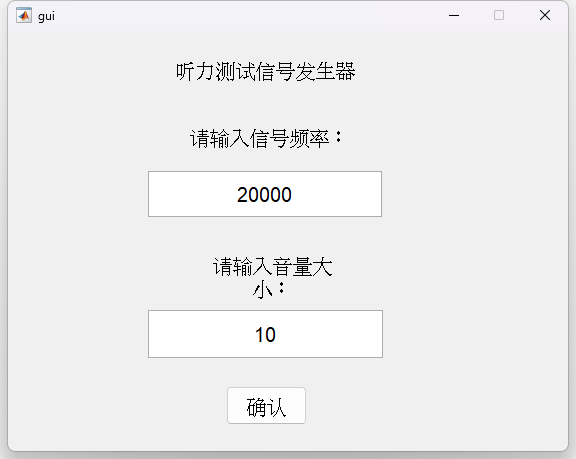
\includegraphics[width=\linewidth]{images/1_Application/hear_test.png}
        \caption{听力测试信号发生器a}
    \end{minipage}
    \hfill
    \begin{minipage}[!h]{0.48\textwidth}
        \centering
        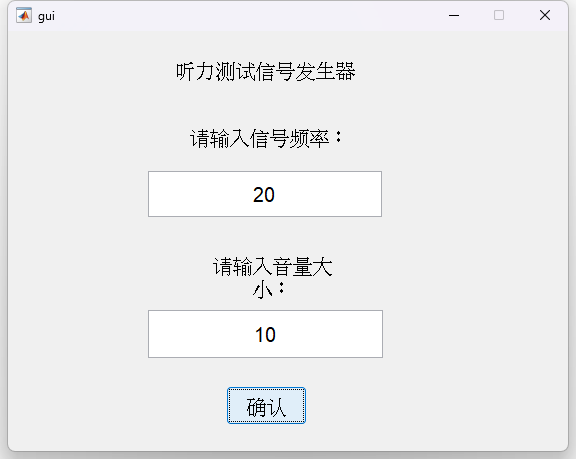
\includegraphics[width=\linewidth]{images/1_Application/hear_test2.png}
        \caption{听力测试信号发生器b}
    \end{minipage}
\end{figure}

在测试过程中,可以发现本人能听见的信号频率范围大概在20Hz到20000Hz左右

\newpage
\bibliographystyle{unsrt}
\bibliography{bibliography/exp2}

\end{document}